\subsection{Creating Rapport Agent using Data-Driven Based Approaches}
\label{sub:sec:datadrivenbasedAgents}

Rule-based systems are not easily scalable seeing that it is impossible to program an agent to handle every possible situation and outcome, especially when interacting with the unpredictability of human behaviour. Therefore, some scenarios may benefit of having agents capable of adapting to changes in the external world and act accordingly using data-driven models. We consider data-driven systems, or \ac{ML}-based systems, as systems that use data collected from studies to train \ac{ML} classifiers and generate appropriate social behaviours.

Mohammad et al., propose a model for interactive robots that can learn how to interact naturally with human conversational partners in different environments and contexts~\cite{Mohammad2010} using unsupervised learning. One of the tested successful scenarios was learning how to apply backchannels in a dyadic setting with a human instructor. According to their results, as expected, the system performs better than the traditional rule-based, however, there is no comparison regarding the traditional supervised learning approaches.

Cakmak, Thomaz and colleagues have been researching the potential of active learning on agents that actively seek information and fill gaps in their knowledge, potentially improving their performance~\cite{Chao2010, Cakmak2010, Cakmak2012, Thomaz2006}. In their studies, they noticed that people who better understand the agent's queries are able to train the model with ``perfect accuracy relatively quickly'' and had more confidence on the trained model performance~\cite{Chao2010}. However, previous work has been more focused on learning task related information and not, as intended in the present document, learning better interactional models to build and maintain rapport.

Current literature on rapport and virtual agents, uses \ac{CRF}~\cite{Buschmeier2011}, \ac{SVM}~\cite{Kok2012}, and \ac{RL}~\cite{Thomaz2006} as classifiers. However every author suggests exploring \ac{RL} algorithms, such as Q-learning (detailed in Section~\ref{subsec:ReinforcementLearning}) to learn human social behaviours~\cite{Thomaz2006, Kok2012, Zhao2014, Papangelis2014, Blumberg2002, Andrist2015}. 

Moreover, it is important to properly design the experiments to correctly collect data. For example, Thomaz et al., developed an agent using \ac{RL} learning \cite{Thomaz2006}. During the experiment, despite asking the humans not to provide feedback (only guidance), they influenced the results. As the author describes ``people use the reward signal to give anticipatory rewards, or future directed guidance for the agent''.

\subsubsection{Virtual Rapport 2.0} \hspace*{\fill} \\
\label{sub:sec:virtualrapport2}

Huang et al., developed a short-term rapport agent to enhance mutual attention and coordination using backchannels through a data-driven approach that takes into account context-specific response models in a dyadic conversational setting~\cite{Buschmeier2011}. The model determines the best suitable timings to generate specific backchannel behaviours and turn-taking opportunities according to the perceptual state observed.

%%%%%%%%%%%%%%%%%%%%%%%%%%%%%%%%%%%%%%%%%%%%%%%%%%%%%%%%%%%%%%%%%%%%%%%%%%%%%%%%%%%%%

\paragraph{\textbf{System description}}

Following Figure~\ref{fig:virtualrapport2System}, the system contains the following modules:
\begin{itemize}
	\item \textbf{\textit{Perception}}: analyses human speaker's behaviour in real time;
	\item \textbf{\textit{Response Models}}: predicts timing of backchannel feedback and end-of-turn opportunities in real time using information from the environment and from the agent itself. It also decides which behaviour to generate;
	\item \textbf{\textit{Generation}}: generates the output from the response models;	
	\item \textbf{\textit{Consensus Data}}: contains data collected from Rapport 06-07 dataset and Self-disclosure data-set (\url{http://rapport.ict.usc.edu}) using \ac{PCS}. The data contains dyadic interactions between a human speaker telling a story and human silent listener.
\end{itemize}

\begin{figure}[hbt]
  \centering
  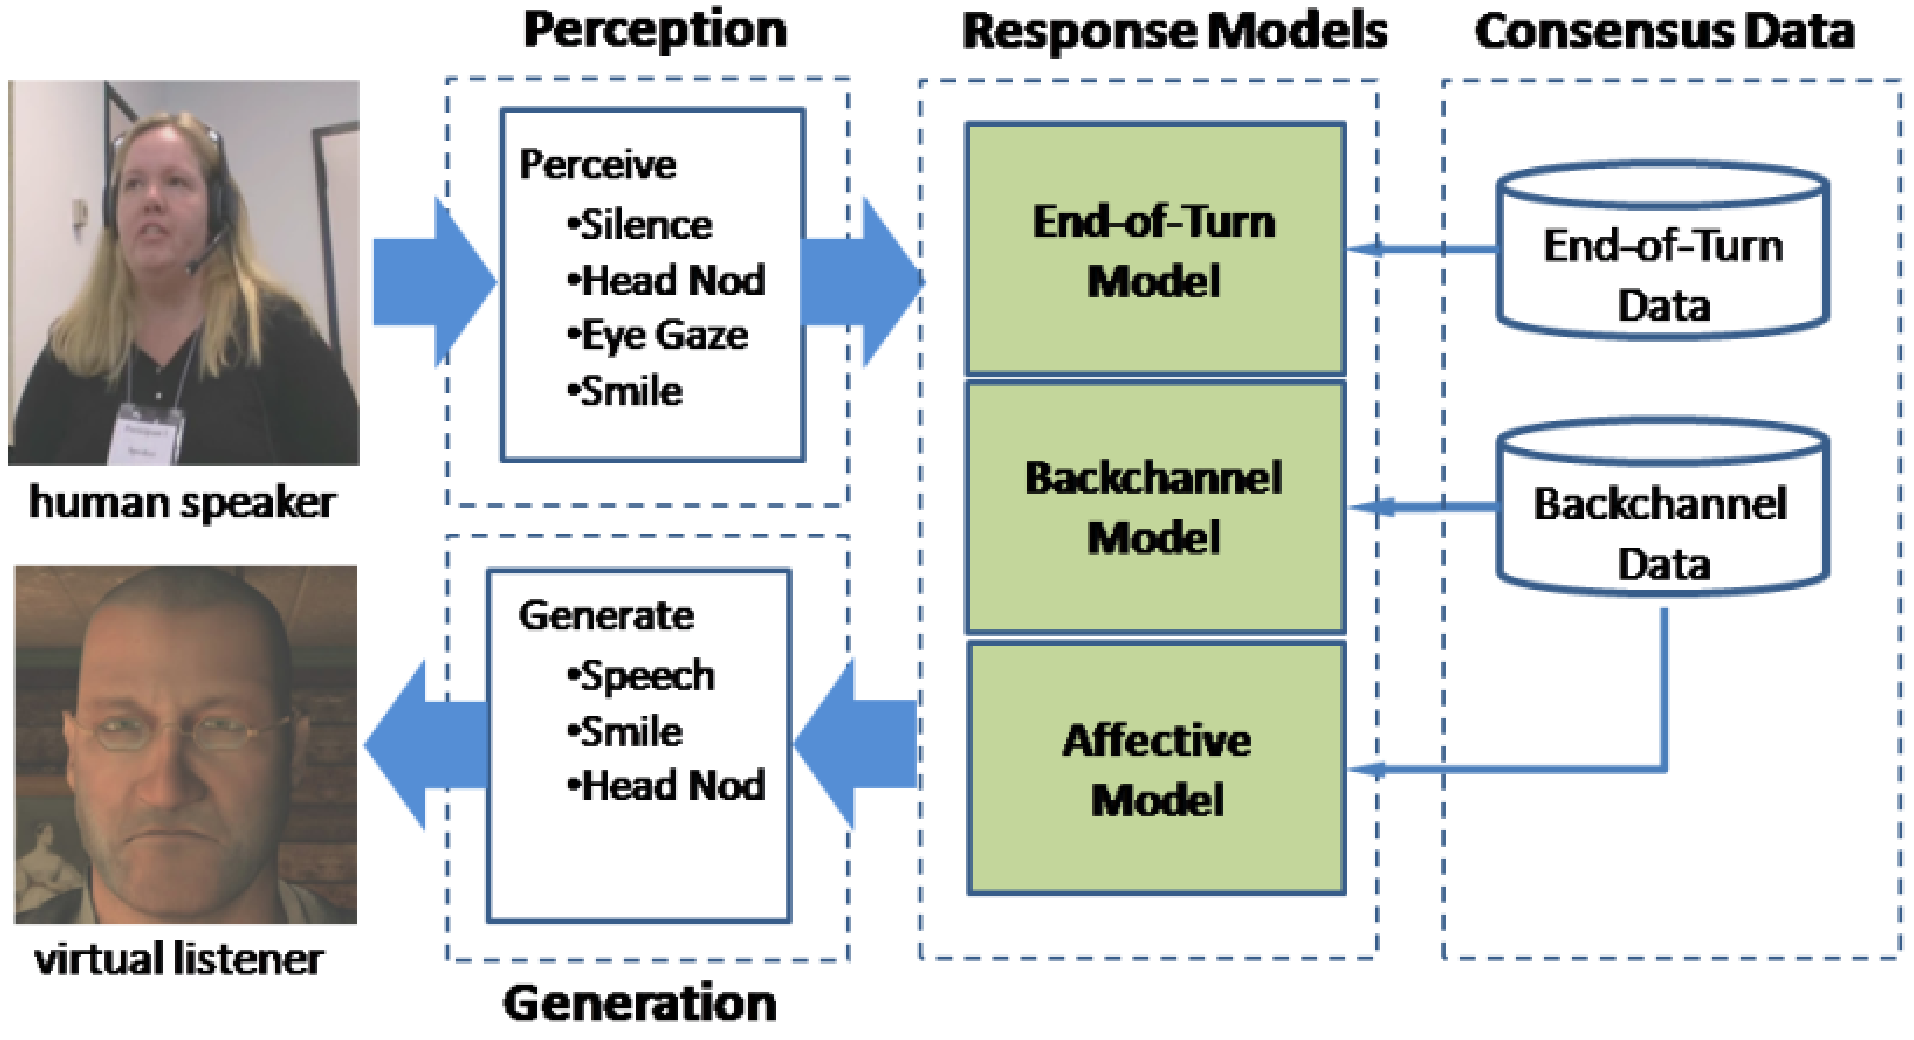
\includegraphics[width=0.8\textwidth]{images/VirtualRapport2_System.png}
  \caption{Architecture of Virtual Rapport 2.0: The \textit{Perception} module analyses human behaviour in real time. \ac{PCS} data is used to create the \textit{Response Models} module. Lastly, the output of the models is generated by the \textit{Generation} module. From~\cite{Buschmeier2011}.}
  \label{fig:virtualrapport2System}
\end{figure} 

As depicted in Figure \ref{fig:virtualrapport2System} there are three models in the \textit{Response Models} module: \textit{End-of-turn}, \textit{Backchannel}, and \textit{Affective}.

The first model, \textit{end-of-turn}, using a rule-based approach, identifies turn-taking opportunities by analysing the current speaker's non-verbal behaviours. For example, if the human interrupts the virtual agent, the agent stops, yields his turn and, says ``I am sorry, keep going'' while showing a facial expression~\cite{Buschmeier2011}.

The second model, \textit{Backchannel}, is \ac{ML}-based (using forward-only inference \ac{CRF} for real-time predictions) and trained using the Rapport 06-07 dataset. It is capable of predicting when and how to give non-verbal feedback.

The last model, \textit{Affective}, analyses facial feature points in real time and detects whenever the speaker is smiling.
 
During the interaction, the three response models are used in conjunction to decide whenever it is appropriate to generate a backchannel. If the speaker is smiling (according to the \textit{Affective} model) and if it is a good opportunity to generate a backchannel (according to the \textit{Backchannel} model) then a head nod (one of the three identified in their studies) is generated accompanied by a smile.

%%%%%%%%%%%%%%%%%%%%%%%%%%%%%%%%%%%%%%%%%%%%%%%%%%%%%%%%%%%%%%%%%%%%%%%%%%%%%%%%%%%%%%%%

\paragraph{\textbf{Evaluation}}
The developed virtual agent interacted with the human subjects in a interview environments in which the former was the interviewer and the later the interviewed. With the goal of comparing the developed system with the previous version~\cite{Gratch2006}, the evaluation measured the following dimensions: rapport (five-item social presence scale~\cite{Bailenson2001}), overall naturalness, backchannel feedback and end-of-turn prediction.


%%%%%%%%%%%%%%%%%%%%%%%%%%%%%%%%%%%%%%%%%%%%%%%%%%%%%%%%%%%%%%%%%%%%%%%%%%%%%%%%%%%%%%%%

\paragraph{\textbf{Discussion}}
The results demonstrates a significant improvement over the previous version. Over 90\% of the users preferred the Virtual Rapport 2.0 rapport agent over the previous rule-based system~\cite{Gratch2006, Morency2008}. The timing's precision and recall are much better, leading to a better synchronism and perceived naturalness from the user during the interaction. According to the authors, the data-driven design, the much richer set of emotions capable of mimicking smiles, and the generation of more natural head gestures might explain the overall better results on the stronger feelings of rapport.

To conclude the most relevant aspects of the system are:
\begin{itemize}
	\item Corpus based approach;
	\item Identification of different head nods patterns;
	\item Duality of \ac{ML}-bases decision and smile to generate backchannel behaviour;
	\item Creative strategy for handling interruptions.
\end{itemize}
\subsubsection{\acl{IPL}} \hspace*{\fill} \\
\label{subsec:IterativePerceptualLearning}

Kok et al., developed an iterative data-driven rapport model focused on generating timings for backchannel behaviours in a dyadic conversational setting~\cite{Kok2012}. The learning stage is iterated several times, each one is more refined and capable of representing generalised behaviours than the previous one. 

Usually, corpus-based backchannel models retrieves negative samples from random moments in the interaction that do not overlap with the positive samples marked in the corpus~\cite{Kok2012}. However, this approach potentially leads to greater number of false negatives by not taking into account that social signals are optional and a reflection of the listener's personality. Therefore different behaviour from the corpus can also be recognised as socially appropriate. In order to tackle this issue, \ac{IPL}, generates social signals and uses perceptual (subjective) evaluation to identify the moments in the interaction that are perceived as socially appropriate and inappropriate.


%%%%%%%%%%%%%%%%%%%%%%%%%%%%%%%%%%%%%%%%%%%%%%%%%%%%%%%%%%%%%%%%%%%%%%%%%%%%%%%%%%%%%
\paragraph{\textbf{System Description}}

Following the representation of the \ac{IPL} system in Figure~\ref{fig:ipl_system}, the system starts with an initial \ac{ML} model (yellow area) that is trained using the corpus-based mentioned. From the corpus~\cite{DeKok2011} it was extracted three types of features: prosody (112 features), speaking (1 feature) and looking (1 feature). After the first subjective evaluation, the negative samples are discarded and replaced by the ones rated by the users. Then, through several iterations of generation  (pink areas), evaluation (blue areas), and learning (green areas) the model is refined and its understanding regarding proper timings for social behaviour evolves.

\begin{figure}
	\centering
	\includegraphics[width=0.3\textwidth]{images/IPL_system.png}
	\caption{Schematic representation of the \ac{IPL} framework. The generation, evaluation and learning stage are shown in pink, blue and green, respectively. From~\cite{Kok2012}.}
	\label{fig:ipl_system}
\end{figure}

%In the generation stage, according to the current model and the partner's behaviour,  

During the generation, non-verbal behaviours are computer generated according to the \ac{ML} classifier and the feature vectors created from the partner's behaviour at a given instance. Then, during the evaluation, using \ac{PCS}~\cite{Huang2010}, multiple subjects evaluate the generated behaviours by pressing a \textit{Yuck} button whenever they would rate the agent's behaviour as socially inappropriate \cite{Poppe2011}. Finally, during the final stage (learning) the retrieved positive and negatives samples are used to train the classifier.

%%%%%%%%%%%%%%%%%%%%%%%%%%%%%%%%%%%%%%%%%%%%%%%%%%%%%%%%%%%%%%%%%%%%%%%%%%%%%%%%%%%%%
\paragraph{\textbf{Evaluation}}

In the evaluation, in each iteration, the authors compared the traditional corpus-based with the iterative approach on face-to-face conversations between the \ac{IPL} agent (listener) and a human subject (speaker) using precision (Equation~\ref{eqn:precision}), recall (Equation~\ref{eqn:Recall}), and perceptual evaluation (\textit{Yuck} button). The experiment lasted for 4 iterations, and the corpus-based system and \ac{IPL} system were trained using the same interactions. The stimuli was a speaker's video from the corpus with a synchronised animated listener capable of only nodding his head while making utterances. 

%%%%%%%%%%%%%%%%%%%%%%%%%%%%%%%%%%%%%%%%%%%%%%%%%%%%%%%%%%%%%%%%%%%%%%%%%%%%%%%%%%%%%
\paragraph{\textbf{Discussion}}

Human subjects perceived the \ac{IPL} virtual agent's backchannels as natural. However, the system was limited because it lacked other relevant features to manage rapport, e.g., mutual gaze, smile, and head angles. This led to, as the author describes, ``a rapid saturation of the model''. Additionally, the authors recommend avoiding \ac{SVM} models because they are not sequential (do not analyse sequential patterns).
 
To conclude there are several relevant positive aspects from the model to the proposed solution:
\begin{itemize}
	\item Iterative approach that is continuously refined and improved;
	\item Perceptual evaluation to identify inappropriate moments in the interactions;
	\item Limiting the listener's perception and increase his focus by limiting the agent's actions;
	\item Generate 25\% more backchannels for the training stage in order to collect more data.
\end{itemize}
\subsubsection{\acl{SAL}} \hspace*{\fill} \\
\label{subsec:AutonomousSensitiveArtificialListeners}

Schröder et al. developed a virtual agent integrated in SEMAINE~\cite{Schroder2010} called \ac{SAL} that has the required capabilities to sustain conversational dialogues and be a good listener~\cite{Schroder2012}.

\paragraph{\textbf{System Description}}

Following the representation of the \ac{SAL} system in Figure~\ref{fig:sensitiveAgent}, the most relevant components are: \textit{Feature extractors}, \textit{Analysers}, \textit{Interpreters}, \textit{Action proposers}, and \textit{Action selection}. The \textit{Feature extractors} component extracts several features such as head gestures, facial features, emotions and, most of all, acoustic features. These features are later analysed by the \textit{Analysers} and \textit{Interpreters} components. The former component analyses non-verbal behaviours and speaker's emotions to produce an estimate of the information's reliability. The later component, given the information available, returns the best state representation for the user, dialogue and agent. Following this, several \textit{Action proposers} will propose an action, in parallel, given previous information. Following, the \textit{Action selection} component selects the action with the highest estimated quality, and lastly, the \textit{Behaviour generator} generates the desired action (utterances and facial animations).

\vspace{-3mm}
\begin{figure}
	\centering
	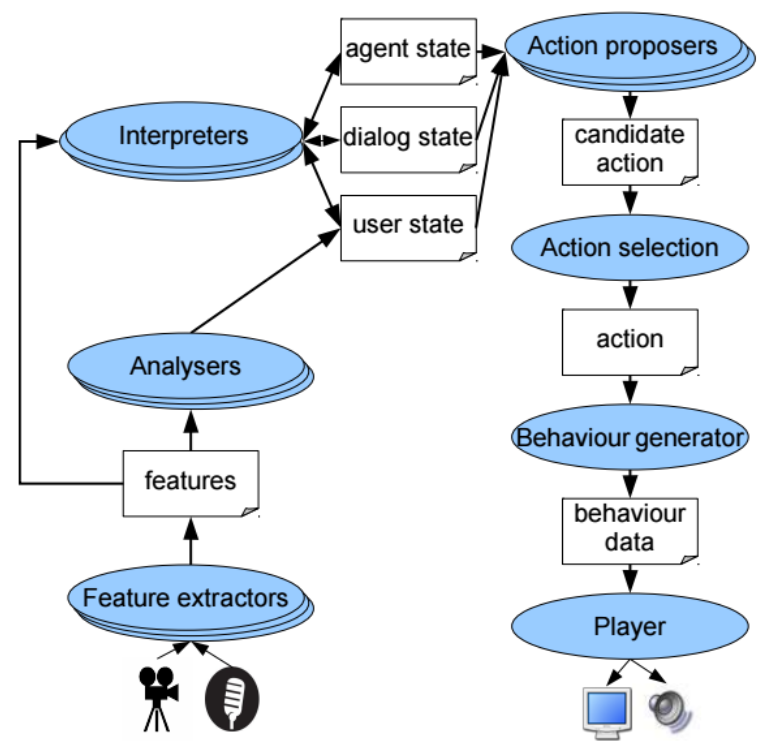
\includegraphics[width=0.5\textwidth]{images/SensitiveAgent.png}
	\caption{\acl{SAL} conceptual architecture. From~\cite{Schroder2012}.}
	\label{fig:sensitiveAgent}
\end{figure}
\vspace{-7mm}

The agent is capable of identifying whether it should be in listener or in speaker mode. This is relevant as the \textit{Action selection} component gives more priority over speaker's actions. An example speaker action would be  saying ``Well?'' or ``Go on, tell me your news!'' after a long pause. In addition, in listener mode, the \textit{Action selection} component chooses the most appropriate backchannel to be produced according to the emotions and interest level estimated from the user.

\paragraph{\textbf{Evaluation}}

The objective was to evaluate if emotion-related abilities influence the quality of human interactions. Firstly the users, with minimal \ac{HRI} experience, receive a introductory briefing on the available personalities they can interact with (4 in total). Then, they can interact twice with each available personality one with the expressive agent, the other with the affective features of the output disabled (randomly). The user interacts with the \ac{SAL} agent's presented in a computer screen (only the face is rendered), using the available cameras and microphones.

\paragraph{\textbf{Discussion}}
There is evidence that expressive abilities may substantially impact the interactions between humans and agents by denoting that flow and perceived engagement was much higher in the emotional \ac{SAL} than in the control environment. Compared with previous described systems, it is one of the most complete models for managing backchannels and turn taking strategies, however, as stated previously in Section~\ref{subsec:Rapport}, attentiveness and coordination are not enough to build rapport, it is also necessary to stimulate positivity which this system does not cover. To conclude, the most relevant aspects of the systems are:

\begin{itemize}
	\item Generate good listeners without understanding semantically what it is being said;
	\item Parallel independent action proposers that uses both rule and \ac{ML} approaches;
	\item Dedicated dialogue management models;
	\item Covers several users affective states by modelling distinct characters.
\end{itemize}